This chapter describes the \cgal's package for the extraction of
ridges on meshes.  Given a smooth surface, a ridge is a curve along
which one of the principal curvatures has an extremum along its
curvature line. Ridges are curves of {\em extremal} curvature and
therefore encode important informations used in segmentation,
registration, matching and surface analysis.  Based on the results of
the article \cite{rr}, we propose several algorithms to identify and
extract different parts of this singular ridge curve and some of its
singularites on a surface given as a mesh.


\subsection{Overview}
%%%%%%%%%%%%%%%%%%%%%%

2 main versions

\begin{itemize}
\item
non-topologically oriented: we output several lists of ridges which
are polylines, each list associated to a type: crest min/max,
ellip/hyper, red/blue.

each line has a weight enabling interactive filtering for the visu

\item
topologically oriented : we output a list of umbilics and some lists
of ridges outside umbilic patches, turning points?
\end{itemize}


%%%%%%%%%%%%%%%%%%%%%%%
\section{Introduction}
\label{sec:intro}
%%%%%%%%%%%%%%%%%%%%%%%

\subsection{Ridges of a smooth surface}
%%%%%%%%%%%%%%%%%%%%%%%%%%%%%%%%%%%%%%%

A comprehensive description of ridges can be found in
\cite{ip-nss-71,hgyg-ttdpf-99,ip-gd-01}, and in the sequel, we just
introduce the basic notions so as to explain our algorithms.
Consider a smooth embedded surface, and denote $k_1$ and $k_2$ the
principal curvatures, with $k_1\geq k_2$. Umbilics are the points
where $k_1=k_2$.  For any non umbilical point, the corresponding
principal directions of curvature are well defined, and we denote them
$d_1$ and $d_2$. In local coordinates, we denote $\langle , \rangle$
the inner product induced by the ambient Euclidean space, and $dk_1$,
$dk_2$ the gradients of the principal curvatures. Ridges, illustrated
on Figs \ref{pict:ellipsoid_ridges} and \ref{fig:ridges_ellipsoid},
are defined by:
%%
\begin{definition}
\label{def:ridge-extrema}
A non umbilical point is called
\begin{itemize}
\item
%a blue ridge point if $\langle dk_1,d_1 \rangle=0$,
a blue ridge point if the {\em extremality coefficient} $b_0=\langle
dk_1,d_1 \rangle$ vanishes, i.e. $b_0=0$.

\item
%a red ridge point if $\langle dk_2,d_2 \rangle=0$.
a red ridge point if the {\em extremality coefficient} $b_3=\langle
dk_2,d_2 \rangle$ vanishes, i.e. $b_3=0$.

\end{itemize}
\end{definition}
%We denote $b_0=\langle dk_1,d_1 \rangle$ and $b_3=\langle dk_2,d_2
%\rangle$, and we call these functions the {\em extremality
%coefficients}. 
%%
Notice that, as the principal curvatures are not differentiable at
umbilics, the extremality coefficients are not defined at such
points. In addition, the sign of the extremality coefficients is not
defined since the principal directions can be oriented by two opposite
unit vectors. Apart from umbilics, special points on ridges are {\em
purple} points, which correspond to intersections between red and a
blue ridges. The previous characterization of ridges involves
third-order differential properties. Using fourth-order differential
quantities, a ridge point can further be qualified as {\em elliptic}
if it corresponds to a maximum of $k_1$ or a minimum of $k_2$, or {\em
hyperbolic} otherwise. Ridges of a given color change from elliptic to
hyperbolic at special points called {\em turning} points.

The calculation of ridges poses difficult problems, which are of three
kinds.

\paragraph{Topological difficulties.}
Ridges of a smooth surface form a singular curve on the surface, with
self-intersections at umbilics (more precisely at so-called 3-ridges
umbilics), and purple points. Moreover, ridges have complex
interactions with curvature lines at turning points. From the
application standpoint, reporting ridges of a surface faithfully
requires reporting umbilics, purple points and turning points.

\paragraph{Numerical difficulties.}
As pointed out above, ridges are characterized and qualified through
third and fourth order derivatives of the surface.  Estimating them
depends on the particular type of surface processed ---implicitly
defined, parameterized, discretized by a mesh--- and is numerically a
difficult task.

\paragraph{Orientation difficulties.}
Since coefficients $b_0$ and $b_3$ depend on a given orientation of
the principal directions, their sign is not well defined.
Practically, tracking the sign change of functions whose sign depends
on the particular orientation of the frame in which they are expressed
poses a problem. In particular, tracking a zero-crossing of $b_0$ or
$b_3$ from sign changes along a curve segment on the surface imposes
to find a coherent orientation of the principal frame at the
endpoints. Given two principal directions at these endpoints, one way
to find a local orientation consists of choosing two vectors so that
they make an acute angle, whence the name {\em Acute Rule}.
%%

\begin{minipage}[c]{.45\linewidth}
\begin{figure}[H] 
\centerline{ 
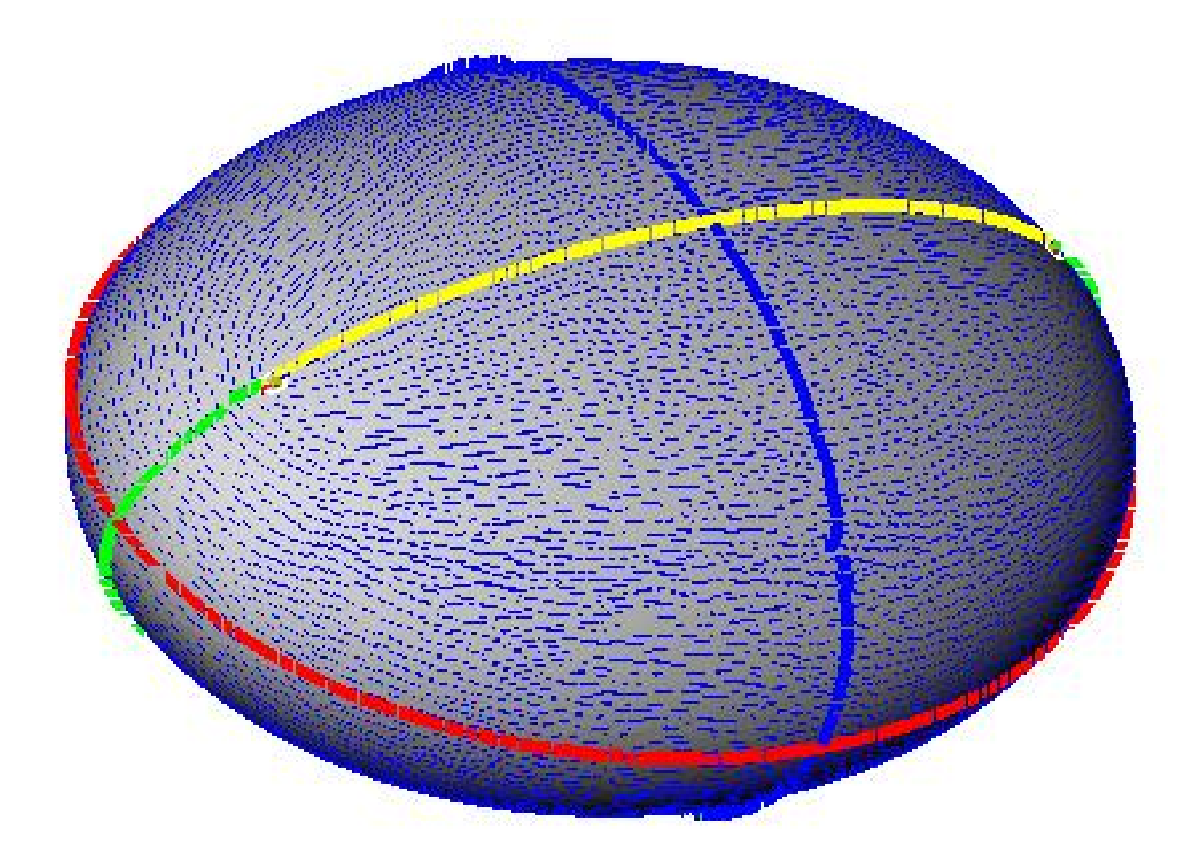
\includegraphics[height=5cm]{Ridges_3/ellipsoid_ridges_mesh}}
\caption{Umbilics, ridges, and principal blue foliation on the
ellipsoid (10k points)}
\label{pict:ellipsoid_ridges} 
\end{figure} 
\end{minipage}
%%
\hfill
%%
\begin{minipage}[c]{.45\linewidth}
\begin{figure}[H] 
\centerline{ 
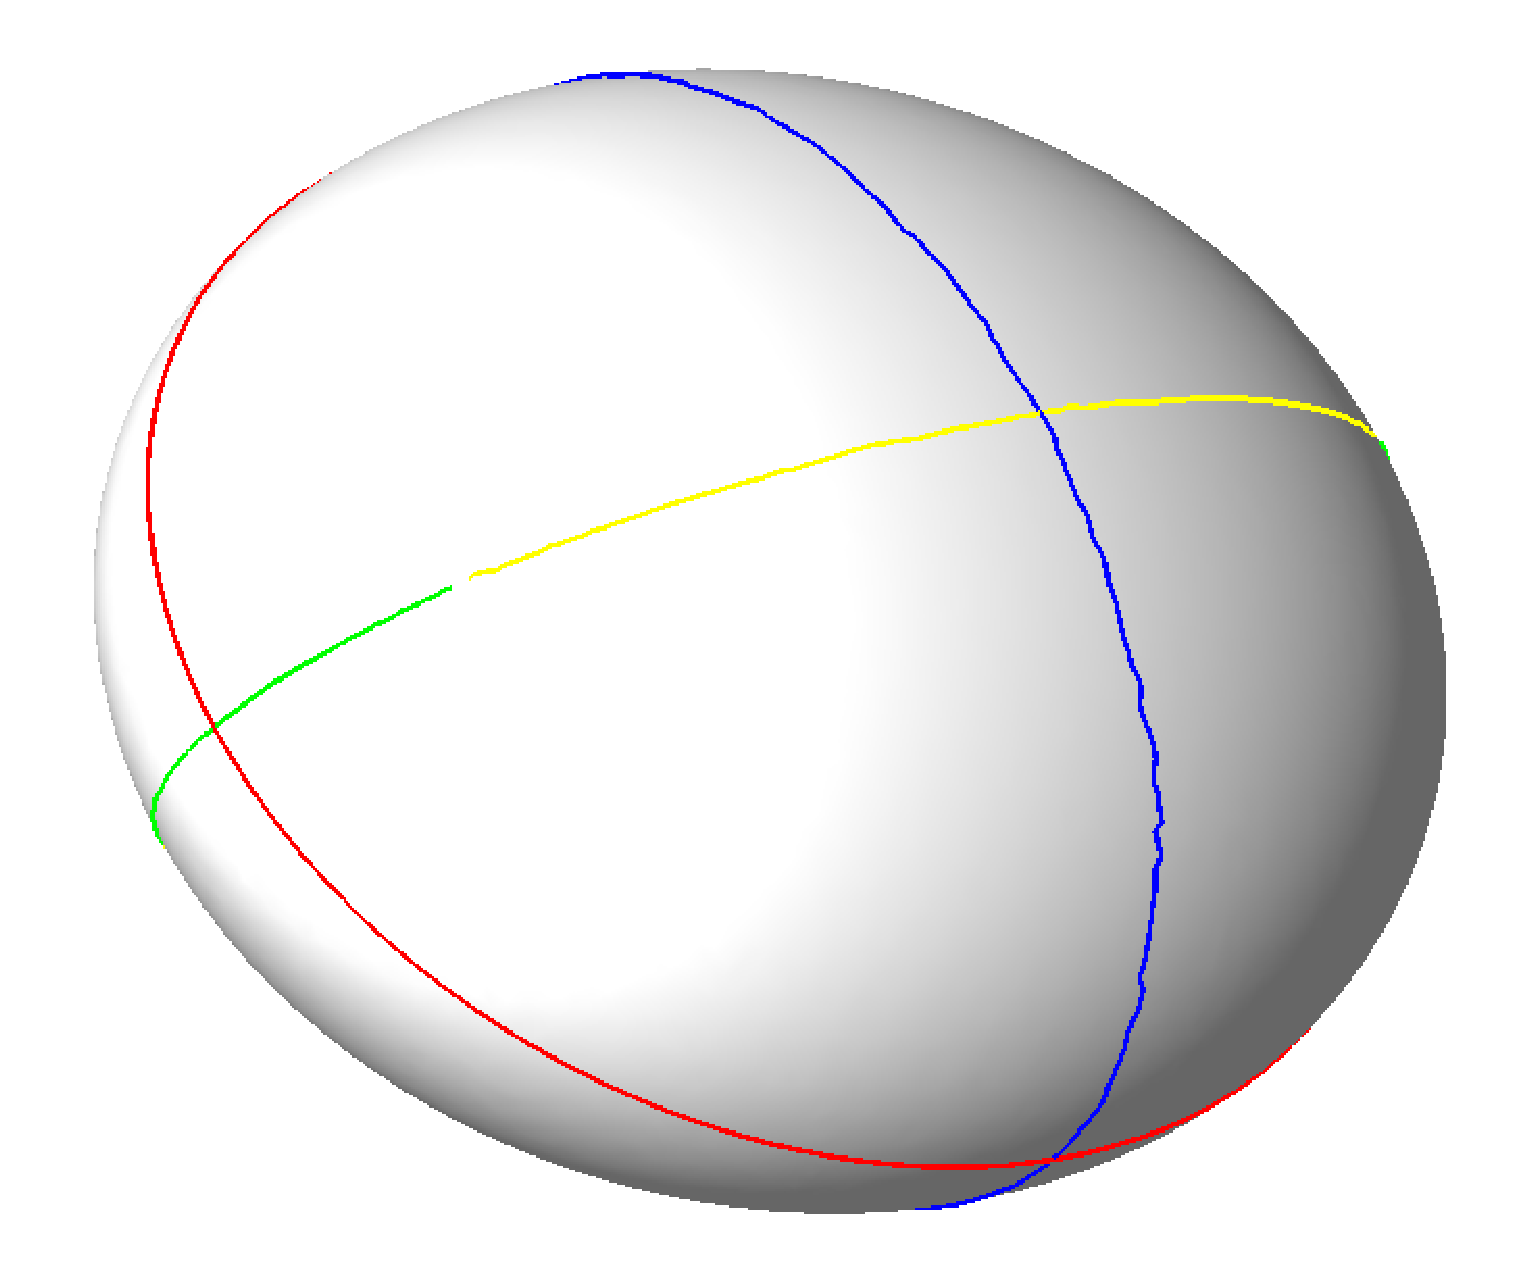
\includegraphics[height=5cm]{Ridges_3/ellipsoid_ridges}}
\caption{Schematic view of the umbilics and the ridges. Max of $k_1$:
blue; Min of $k_1$: green; Min of $k_2$: red; Max of $k_2$: yellow}
\label{fig:ridges_ellipsoid}
\end{figure} 
\end{minipage}



%%%%%%%%%%%%%%%%%%%%%%%
\section{Software Design}
%%%%%%%%%%%%%%%%%%%%%%%


\subsection{Options and interface specifications}
%%%%%%%%%%%%%%%%%%%%%

\subsection{Template parameters}
%%%%%%%%%%%%%%%%%%%%%%%%%%%%%%%%%

\subsection{Output}
%%%%%%%%%%%%%%%%%%%%



%%%%%%%%%%%%%%%%%%%%%%%%%%%%%%%%%%%%%%%%%%%%%%%%%%%%%%%%%%%%%%%%%%%%%%%%%%%%
\section{Examples} 
%%%%%%%%%%%%%%%%%%%%%%%%%%%%%%%%%%%%%%%%%%%%%%%%%%%%%%%%%%%%%%%%%%%%%%%%%%%%
